\documentclass[border=6pt]{standalone}
\usepackage[T1]{fontenc}
\usepackage{lmodern}
\usepackage{amsmath,amssymb,bm}
\usepackage{xcolor}
\usepackage{tikz}
\usetikzlibrary{arrows.meta,positioning,fit,backgrounds,calc}
\definecolor{swinc}{HTML}{2166AC}
\definecolor{cnnc}{HTML}{1B7837}
\definecolor{decc}{HTML}{E66101}
\definecolor{botc}{HTML}{B2182B}
\definecolor{headc}{HTML}{762A83}
\newcommand{\code}[1]{\texttt{\detokenize{#1}}}
\begin{document}
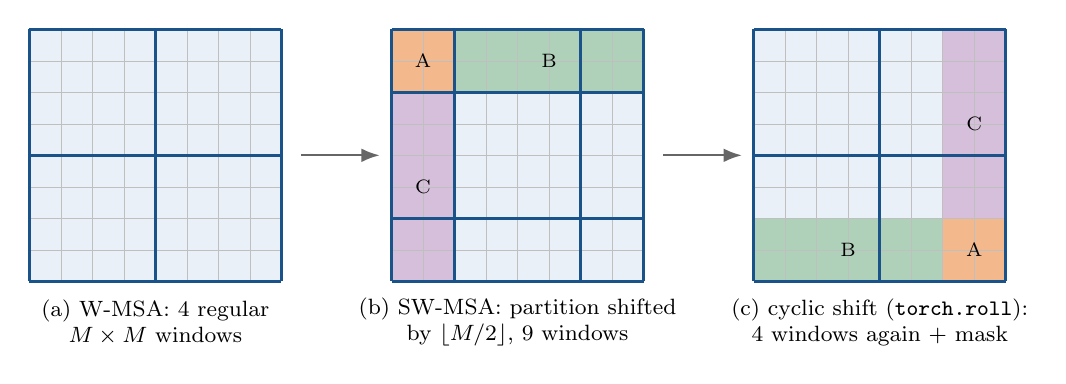
\begin{tikzpicture}[font=\footnotesize, >=Latex]
\def\s{0.4}
\newcommand{\region}[5]{\fill[#5] (#3*\s,-#1*\s) rectangle (#4*\s,-#2*\s);}
\newcommand{\gridlines}{\draw[black!25, very thin] (0,0) grid[step=\s] (8*\s,-8*\s);}

\begin{scope}
  \region{0}{8}{0}{8}{swinc!10}
  \gridlines
  \foreach \t in {0,4,8} {\draw[very thick, swinc!80!black] (\t*\s,0) -- (\t*\s,-8*\s); \draw[very thick, swinc!80!black] (0,-\t*\s) -- (8*\s,-\t*\s);}
  \node[align=center] at (4*\s,-9.3*\s) {(a) W-MSA: 4 regular\\ $M\times M$ windows};
\end{scope}

\begin{scope}[xshift=4.6cm]
  \region{0}{8}{0}{8}{swinc!10}
  \region{0}{2}{0}{2}{decc!45}
  \region{0}{2}{2}{8}{cnnc!35}
  \region{2}{8}{0}{2}{headc!30}
  \gridlines
  \foreach \t in {0,2,6,8} {\draw[very thick, swinc!80!black] (\t*\s,0) -- (\t*\s,-8*\s); \draw[very thick, swinc!80!black] (0,-\t*\s) -- (8*\s,-\t*\s);}
  \node at (1*\s,-1*\s) {\scriptsize A};
  \node at (5*\s,-1*\s) {\scriptsize B};
  \node at (1*\s,-5*\s) {\scriptsize C};
  \node[align=center] at (4*\s,-9.3*\s) {(b) SW-MSA: partition shifted\\ by $\lfloor M/2\rfloor$, 9 windows};
\end{scope}

\begin{scope}[xshift=9.2cm]
  \region{0}{8}{0}{8}{swinc!10}
  \region{6}{8}{6}{8}{decc!45}
  \region{6}{8}{0}{6}{cnnc!35}
  \region{0}{6}{6}{8}{headc!30}
  \gridlines
  \foreach \t in {0,4,8} {\draw[very thick, swinc!80!black] (\t*\s,0) -- (\t*\s,-8*\s); \draw[very thick, swinc!80!black] (0,-\t*\s) -- (8*\s,-\t*\s);}
  \node at (7*\s,-7*\s) {\scriptsize A};
  \node at (3*\s,-7*\s) {\scriptsize B};
  \node at (7*\s,-3*\s) {\scriptsize C};
  \node[align=center] at (4*\s,-9.3*\s) {(c) cyclic shift (\texttt{torch.roll}):\\ 4 windows again + mask};
\end{scope}

\draw[->, thick, black!60] (3.45,-1.6) -- (4.45,-1.6);
\draw[->, thick, black!60] (8.05,-1.6) -- (9.05,-1.6);
\end{tikzpicture}
\end{document}
